% ============================================================
%  Extrinsic Is Not One Thing:
%  Recipient Exchangeability in Evolutionary Systems
%  R.-A. Jaen-Garcia, J. Larrey-Ruiz  --  v9, BioSystems
%
%  COMPILACION: pdflatex -> bibtex -> pdflatex -> pdflatex
%  Ya NO se usa biber.  elsarticle carga natbib por su cuenta.
% ============================================================

\documentclass[review,3p,times]{elsarticle}

\usepackage[T1]{fontenc}
% NO cargar lmodern: se carga DESPUES de la clase y gana, con lo que la opcion
% `times` deja de surtir efecto y las fuentes embebidas salen LMRoman en vez de
% NimbusRomNo9L.  Comprobado con pdffonts; quitarlo baja el documento de 38 a
% 30 paginas.
\usepackage{microtype}
% geometry: lo aporta elsarticle
\usepackage{amsmath,amssymb}
\usepackage{booktabs}
\usepackage{array}
\usepackage{graphicx}
% Los \includegraphics van sin extension, asi que sin esto graphicx elegiria el
% PDF.  Cuestan lo mismo (3,25 s el PDF frente a 3,24 s el PNG, pase estable),
% y se compila con las PNG a proposito.  Los PDF siguen ahi para el envio.
\DeclareGraphicsExtensions{.png,.pdf}
\usepackage{xcolor}
\usepackage{enumitem}
% lineno y authblk: los aporta o los sustituye elsarticle
\usepackage{csquotes}

\IfFileExists{orcidlink.sty}{\usepackage{orcidlink}}{\providecommand{\orcidlink}[1]{}}
\newcommand{\aind}{\textsuperscript{1}}

\biboptions{authoryear}

\usepackage{hyperref}
\hypersetup{colorlinks=true, linkcolor=blue, citecolor=blue, urlcolor=blue}
% hyperref mete el bloque \author en los metadatos del PDF, y ahi no puede
% representar \textsuperscript ni \orcidlink.  De ahi salian los seis avisos,
% no de los titulos de seccion.  Se vacian solo para la cadena PDF: lo
% impreso no cambia.
\pdfstringdefDisableCommands{\def\aind{}\def\orcidlink#1{}}

\newdefinition{definition}{Definition}

% ---------------------------------------------------------------
% UNICO PUNTO DE EDICION DE LA URL DEL REPOSITORIO.
% Aparece en la nota al pie de Methods y en Data Availability.
% BioSystems usa revision single anonymized: no hay copia anonima.
% ---------------------------------------------------------------
\newcommand{\repourl}{\url{https://github.com/rauljaengarcia/Extrinsic-is-not-one-thing}}

\begin{document}

\begin{frontmatter}

\title{Extrinsic Is Not One Thing: Recipient Exchangeability in
Evolutionary Systems}

\author{
Ra\'ul-Antonio Ja\'en-Garc\'ia\orcidlink{0009-0004-1273-1422}\aind,
Jorge Larrey-Ruiz\aind\\
{Universidad Polit\'ecnica de Cartagena, Cartagena, Spain}\\
{\small \texttt{raul.jaen@edu.upct.es, jorge.larrey@upct.es}}
}

\setcounter{footnote}{1}
\renewcommand\thefootnote{\arabic{footnote}}
\footnotetext{Universidad Polit\'ecnica de Cartagena. Escuela T\'ecnica
Superior de Ingenier\'ia de Telecomunicaci\'on. Edificio Cuartel de
Antigones. Plaza del Hospital, 1, 30202, Cartagena, Espa\~na.
Corresponding author: Ra\'ul-Antonio Ja\'en-Garc\'ia,
\texttt{raul.jaen@edu.upct.es}}

\begin{abstract}
Whether the supply a lineage receives depends on \emph{who that lineage is},
rather than on what state it is in, is a property of biological organization,
distinct from the question of who operates the supplying rule. A rule is
\emph{recipient-exchangeable} when relabelling recipients' identities and
provenances, holding their states fixed, leaves every allocation unchanged,
and \emph{recipient-partial} otherwise. That is the anonymity condition of
social choice, in the form that holds states fixed, applied to evolutionary
supply. With the intrinsic/extrinsic distinction, recipient exchangeability
gives every rule two independent coordinates.

The distinction separates biological cases ordinarily run together.
Provisioning cued by a state correlating with relatedness is exchangeable;
care directed at individually recognised offspring, or keyed to pedigree, is
not. Ordering eight audited systems by both coordinates yields a partial
order: a free-living microbial population dominates every artificial system
but the digital organism, with which it is incomparable. Conflating
the axes is an error: a breeder reproducing only animals whose trait exceeds a
threshold applies an exchangeable rule, so exchangeability is no criterion for
evolutionary autonomy.

We then build the smallest system in which both can be manipulated
independently. At baseline the four conditions are bit-for-bit identical:
neither coordinate has a dynamical signature until the intervention that
interrogates it. Running the framework found two
defects in it, reported rather than repaired: the contrast is not bounded
above, and the coordinate does not distinguish a rule that excludes a lineage
from one that partitions it.
\end{abstract}

\begin{keyword}
recipient exchangeability \sep anonymity \sep evolutionary transitions \sep
biological organization \sep kin recognition \sep digital evolution \sep
evolvable AI
\end{keyword}

\end{frontmatter}

% ============================================================
\section{Introduction}
% ============================================================

Every evolving lineage is supplied by something it does not wholly control:
nutrients, hosts, habitat, the machinery of replication. A question about the
organization of that supply, and not about its quantity, is whether what a
lineage receives depends on \emph{who that lineage is}. A patch of nitrogen
does not know which clone is drawing on it, and would serve any other clone in
the same physiological state identically. A host that recognises specific
symbiont partners does know, and would not. Both lineages may be equally
dependent; they differ in whether the rule governing the supply turns on the
recipient's identity. That difference is a property of the organization of the
relationship, and it is not the same question as who operates the rule---the
patch and the host are both external to the lineage they supply.

We call the property \emph{recipient exchangeability}. A rule is
recipient-exchangeable when relabelling the identities and provenances of
recipients, holding their causal states fixed, leaves every allocation
unchanged, and recipient-partial otherwise. This is not a new mathematical
condition: it is the \emph{anonymity} axiom of social choice and mechanism
design \citep{may1952,moulin2003}. The contribution is its application to
evolutionary supply, as a dimension independent of control, together with an
interventional method for establishing how much a system relies on it.

Making the condition explicit separates biological cases that are ordinarily
run together under a single heading. Kin-directed behaviour is usually cited
as the paradigm of a specific, non-anonymous interaction. Under the definition
it mostly is not. Provisioning triggered by a state cue that correlates with
relatedness---a recognition allele, a shared odour, the local composition of
the population---is exchangeable, because any individual presenting the same
cue would be served identically. What is partial is care directed at
individually recognised offspring, or keyed to pedigree rather than to
anything about the recipient's state. The same applies across the standard
list of counterexamples: frequency dependence operates on the composition of
states, host--parasite specificity matches genotypes, and mate choice responds
to phenotype, so all three remain exchangeable, while individual recognition
backed by memory and stable dominance relations do not. Sorting the cases this
way is a result of the framework, not a caveat on it.

The second coordinate is the one the literature already has. \citet{taylor2019}
distinguishes evolutionary functions implemented \emph{intrinsically}, by
mechanisms within the evolving system, from those implemented
\emph{extrinsically}. The two coordinates are independent, and conflating them
is an error in a specific direction: a breeder who reproduces only animals
whose milk yield exceeds a threshold applies a perfectly exchangeable rule,
since swapping two animals with identical traits swaps the outcome with them.
Domestication is a fact about who sets the criterion and executes the loop.
Exchangeability is therefore not a criterion for evolutionary autonomy, and
\S2.4 shows that neither axis reduces to the other in either direction.

Artificial systems are where the second coordinate becomes measurable and
manipulable, and where it has recently begun to move. Self-replicating
programs mutate, compete and form ecological relationships
\citep{ray1991,ofria2004,lehman2020}, recent work pursues models in which
reproduction and development proceed without a predefined guide
\citep{utimula2025}, and the structures that can carry heritable variation now
extend to the parameters of large language models \citep{zhang2026}. Whether
this amounts to a major evolutionary transition is disputed:
\citet{muller2026} distinguish ``breeder'' regimes, in which humans set
fitness and control reproduction, from ``ecosystem'' regimes in which fitness
is emergent; \citet{boudry2026} replies that evolvable AI is
\emph{domesticated, not feral}; \citet{mullerreply2026} answer that the threat
is too grave to be left to intuition, while \citet{rana2026} call for
operational thresholds and \citet{mullerthresholds2026} propose autonomous
replication, a von~Neumann-like complexity threshold, and an integrated
Darwinian threshold. That exchange is an instructive test case, because what
runs through all of it is Taylor's axis alone. Consider a researcher who
allocates compute to a particular population because it is their experiment,
and who would not allocate it to an uninvited lineage at any price, against a
cloud market that rents to whichever account pays. Both are extrinsic, both
may be indispensable, and the axis in current use does not separate them. A
lineage supplied entirely by rules of the second kind stands to its suppliers
as an organism stands to an ecosystem, which is compatible with total
dependence---organisms require oxygen---while a lineage supplied by rules of
the first kind stands in the position of an organism in a laboratory.

% ============================================================
\section{Two Axes}
% ============================================================

\subsection{One object, two coordinates}

Let $D$ be a focal evolving system. Let $\sigma$ be an \emph{allocation or
interaction rule} bearing on one of $D$'s evolutionary functions---a
mechanism that determines what some recipient gets, undergoes, or does. We
do not require $\sigma$'s provider to be external; internal mechanisms are
rules too, and the point of the framework is that both coordinates apply to
the same object.

The first coordinate is Taylor's:
\begin{equation}
C(\sigma)=
\begin{cases}
\mathrm{I} & \text{mechanism instantiated within } D,\\
\mathrm{E} & \text{mechanism instantiated outside } D .
\end{cases}
\end{equation}

The second is defined in \S2.2. Both are properties of $\sigma$, which
matters because an evolutionary function is often served by more than one
rule, and the rules need not share coordinates. \S4.5 gives a real case in
which they do not.

We use Taylor's decomposition of the functions, and are deliberately
faithful to it, since the analysis below turns on the boundary he draws.
Generation $G$ maps hereditary description to expressed phenotype.
\emph{Evaluation} $E$ determines lifetime, whether and when reproduction
occurs, how much of it there is, and the mate pool. \emph{Reproduction with
variation} $R$ is the operation that produces the offspring's hereditary
description. Whether an individual reproduces is therefore $E$, not $R$; a
point we would otherwise get wrong in \S4.1. Where infrastructure is at
issue we add maintenance $M$, resource acquisition $Q$ and habitat
persistence $H$.

\subsection{Recipient exchangeability}

Let $X=(x_1,\dots,x_n)$ be a configuration of candidate recipients, where
each $x_i=(z_i,\ell_i)$ comprises a \emph{state} $z_i$---genotype or
parameters, expressed phenotype or behaviour, holdings of transferable
resources, spatial or network position, relational attributes such as
kinship---and an \emph{identity label} $\ell_i$ recording who it is, where
it came from, and what it belongs to, including membership in a particular
population or experiment. Write $\sigma(X)_i$ for what recipient $i$
receives. Let $P_\pi$ permute labels only, leaving states in place, so that
$P_\pi X$ has $i$-th recipient $(z_i,\ell_{\pi(i)})$.

\begin{definition}[Recipient exchangeability]
$\sigma$ is \emph{recipient-exchangeable} if for every permutation $\pi$ of
identity labels and every admissible configuration $X$,
\begin{equation}
\sigma(P_\pi X)_i \;=\; \sigma(X)_i \qquad \text{for all } i .
\label{eq:exch}
\end{equation}
We write $A(\sigma)=0$ for a rule satisfying \eqref{eq:exch} and
$A(\sigma)=1$ for one violating it, calling the latter
\textbf{recipient-partial}.
\end{definition}

The condition reads as a counterfactual: \emph{if this same entity had a
different identity or provenance, would it be treated the same?} Permuting
labels rather than entities is what makes the definition non-vacuous:
permuting entities would require states to coincide, which in a real
population they do not, so no non-trivial permutation would exist and every
rule would satisfy the condition trivially.\footnote{We take $A$ to be
binary. A graded version,
$A_\mu(\sigma)=\mathbb{E}_{X\sim\mu,\pi\sim\Pi}\,d\!\left(\sigma(P_\pi X),\sigma(X)\right)$,
requires a distribution over configurations, a distribution over
permutations and a metric on allocations, none with an obvious canonical
choice. We leave it to future work rather than report a number we cannot
defend.}

Three consequences follow.

\paragraph{Technical identity is not partiality}
Accounts, wallet addresses, process identifiers and API keys are labels, and a
rule using them is not thereby partial. A market paying whichever address holds
the tokens satisfies \eqref{eq:exch}; one paying a specific address because of
whose it is does not.

\paragraph{The biological counterexamples remain exchangeable}
Natural selection is not always blind---frequency-dependent selection, kin
recognition, host--parasite coevolution and mate choice are all specific---but
under \eqref{eq:exch} they are exchangeable all the same, because frequency
dependence operates on the composition of states, kinship is a relational
attribute of state, coevolutionary specificity matches genotypes and mate
choice responds to phenotype. The genuinely partial cases in
nature---individual recognition backed by memory, and stable dominance
relations in which the rule tracks the individual rather than the
rank---are comparatively rare and usually internal to the focal lineage.

\paragraph{Membership may be state or label, and the difference is
principled}
Saying simply that membership is a label is too blunt: belonging to the local
group occupying a patch, or holding a credential acquired by interaction, are
ecological facts about an entity. We adopt an explicit criterion:

\begin{quote}
A property belongs in $z$ if it can in principle be acquired, lost or
changed through the ordinary dynamics available to candidate recipients. It
belongs in $\ell$ if changing it amounts only to changing nominal identity,
provenance or externally assigned membership while holding the recipient's
causal state fixed.
\end{quote}

\emph{Dynamically attainable} membership is state; \emph{nominal} membership is
label. Holding tokens is state, because an entity can come to hold them; being
one of the individuals the framework instantiated at $t=0$ is label, because
nothing an outsider does can make it true. A rule whose domain is nominal
membership is therefore partial, while one whose domain is an attainable
condition is not. This also constrains Arm~S of \S3.4: the substitute
provider's qualifying condition must be dynamically attainable, or the arm has
de-personalised nothing.

The criterion asks what the rule's \emph{domain} is, not how the property came
to be held, and the two are easily confused. Dominance rank is state, since it
is acquired through interaction; but a rule of the form ``I yield to
\emph{this} individual, the one who beat me'' is anchored to an individual and
not to the rank, and is partial for that reason, while ``I yield to whoever
outranks me'' is anchored to state and is not. Likewise, relatedness is
perceived through cues that are state; but a rule of the form ``I provision
\emph{my own} line'' is anchored to provenance. In each pair the property is
the same and $A$ differs, because what settles $A$ is the domain the rule
quantifies over.

One inference must be blocked here, because it is tempting and wrong.
\emph{Closure is not partiality.} A sealed island, a sterile flask and a
bounded memory arena all have participant sets outsiders cannot join, and none
contains a rule that treats anyone differently for being who they are: there is
no causal path in. Partiality requires an allocator whose supply is conditioned
on the recipient's identity, not merely the absence of an entry route. Where a
closed artificial world is nonetheless partial---and \S4 finds that it usually
is---the reason is a provider who maintains that world \emph{for this
population}, which is a rule about who is served, not a fact about topology. A
population admitting members only by reproduction is not partial at all; that
is how biological populations work.

\subsection{The focal system must be declared}

\eqref{eq:exch} quantifies over recipients and $C$ is defined relative to
$D$, so both require a boundary. The criterion does not dissolve the problem
of where the ancestral system ends; it relocates the boundary from a place
where it cannot
be drawn to a place where it routinely is: we never have to decide what
humanity is or treat it as a monolithic evolutionary agent, but we do have
to declare the focal population, which every evolutionary study does
anyway.

\subsection{The axes are independent}

\begin{table}[ht]
\centering
\small
\caption{The two coordinates are independent. Each cell is occupied, and
the two extrinsic cells are the pair the current debate does not
distinguish.}
\label{tab:2x2}
\begin{tabular}{p{2.4cm}p{5.5cm}p{5.5cm}}
\toprule
 & \textbf{Exchangeable} ($A=0$) & \textbf{Recipient-partial} ($A=1$)\\
\midrule
\textbf{Intrinsic}
& Self-replication in Tierra; a reproductive condition read off the
entity's own state
& Care for individually recognised offspring; provisioning keyed to pedigree
rather than to recipient state\\
\addlinespace
\textbf{Extrinsic}
& Generic fitness function; fitness-proportionate scheduler; open compute
market; a public execution service anyone may invoke; oxygen
& Breeder favouring a named lineage; researcher assigning resources to this
experiment; admission restricted by nominal population identity; an evaluation
trial initiated for this model\\
\bottomrule
\end{tabular}
\end{table}

Two cells in Table~\ref{tab:2x2} do the work, and both are easy to get wrong.

\paragraph{Extrinsic and exchangeable is common, and is not autonomy}
A breeder who reproduces only individuals whose trait exceeds a threshold
applies $\sigma(x)=\mathbb{1}[\,\mathrm{trait}(x)>\tau\,]$, which satisfies
\eqref{eq:exch} exactly, as does a scheduler reproducing $x$ with probability
$f(x)/\sum_j f(x_j)$ on the framework's own clock. Both are paradigm cases of
an external agent determining reproduction by criteria of its own, and both
are exchangeable. Domestication in Boudry's sense, and the breeder regime of
Müller and colleagues, therefore live on Taylor's axis and not on ours.

\paragraph{Intrinsic and partial is ordinary biology}
A mother provisions the offspring she recognises as \emph{hers}, whatever
another's state: the rule is keyed to identity and the mechanism is internal
to the lineage. Kin-directed behaviour cued by state stays exchangeable under
\eqref{eq:exch}. If partiality alone removed autonomy, no lineage with such
care would be evolutionarily autonomous, which is absurd.

It follows that neither coordinate is a criterion for evolutionary autonomy
by itself, and we do not claim that ours is. What we claim is narrower:

\begin{equation}
\boxed{
\begin{array}{c}
\text{A rule bearing on an evolutionary function has two independent properties:}\\[2pt]
\text{whether it is operated from within, and whether it depends on recipient identity.}
\end{array}}
\label{eq:twoaxes}
\end{equation}

Free-living biological populations combine intrinsic generation and
reproduction with evaluation emerging from an environment whose rules are
largely recipient-exchangeable: that configuration requires movement on both
axes, and a system can travel a long way along either while standing still on
the other. It also locates an under-characterised change in increasingly
agentic AI. An agent that rents compute from a market, holds funds in an
account and persists on infrastructure that has no idea who it is receives
extrinsic supply under rules exchangeable in a way a laboratory allocation
never was. That is a real movement, it is not what the debate is measuring,
and by itself it is not autonomy.

\paragraph{What would falsify this}
Table~\ref{tab:2x2} shows the cells can be occupied, not that real systems
occupy them. The thesis fails if the coordinates covary in systems nobody
built to separate them: the empirical motivation for treating them separately
would weaken if intrinsic operation and exchangeable supply reliably covaried
across independently arising rules, since one coordinate would then predict
the other and tracking both would buy nothing. That is an empirical claim and
it is checkable---place
audited systems on the plane and see whether they lie near the diagonal.
Figure~\ref{fig:perfil} is that check. They do not, which is evidence rather
than proof, since eight systems chosen partly for being instructive are not a
sample.

\subsection{A partial, not a total, order}

Because a system is characterised by the coordinates of the rules bearing
on each of its functions, comparisons between systems are governed by a
product order. Write $D_1 \succeq D_2$ when, for every function, $D_1$'s
rules are at least as intrinsic and at least as exchangeable as $D_2$'s.
Many pairs satisfy neither $D_1 \succeq D_2$ nor $D_2 \succeq D_1$: they are
\emph{incomparable}. Where a single function is served by rules of differing
coordinates, as several are in Table~\ref{tab:audit}, we compare it by the
weaker of them on each axis. This is a minimum within one function, not an
aggregation across functions, and needs no weights; it is conservative, in
that it never credits a system with a coordinate one of its rules does not
have. The resulting pair is a lower envelope used for comparison, not a claim
that any rule implements it.

We take incomparability to be the generic case rather than an awkward
residue, and it is the formal content of the paper's complaint. Two distinct
errors are worth separating here. A framework tracking only one coordinate
collapses distinctions between rules that differ on the omitted axis, so that
systems differing in what they depend on are recorded as differing in
degree---but it does not thereby produce a total order, since comparisons
still run over six functions and a product order over six components stays
partial. Any scalar ranking goes further and imposes rankings the joint order
need not support, declaring one system ``more autonomous'' than another when
what is true is that each dominates on a different function. Nothing here
licenses combining the coordinates into a scalar; doing so would require
weights we have no principled way to choose, and would reintroduce exactly the
false rankings the two axes exist to prevent. \S4.7 gives three artificial systems, thirty years apart,
that the order does not rank: two of the pairs are incomparable, and the
third turns on a table entry the sources leave open.

\subsection{A rule's property is not a system's dependence}

The properties defined above belong to rules. Whether an evolving system
\emph{relies} on them is a different question with a different answer.

A provider may apply an unmistakably partial rule that makes no difference
to evolutionary continuity, or that makes it worse: a breeder intervening
in a lineage to its detriment supplies partial support the lineage does not
need. Conversely, a rule may be exchangeable while the system depends on it
absolutely, which is the situation of an organism and its oxygen.

\begin{equation}
\boxed{
\;\text{partiality of a rule}
\;\neq\;
\text{reliance on partial supply}\;
}
\label{eq:neq}
\end{equation}

$A(\sigma)$ characterises the rule and is established by inspection or
permutation test (\S3.1--3.2). $\rho$ characterises how much the partial
component matters to continuity and requires intervention (\S3.5).
Reporting one as though it were the other is the error \eqref{eq:neq}
exists to prevent.

\subsection{Relation to existing work}

\paragraph{Anonymity in social choice and mechanism design}
Condition \eqref{eq:exch} is the anonymity axiom, which \citet{may1952} showed
characterises simple majority rule together with neutrality and positive
responsiveness, and which is standard in fair division and mechanism design
\citep{moulin2003}. It is anonymity in the form that permutes labels while
holding states fixed, rather than permuting the bearers themselves: as \S2.2
sets out, permuting entities would require their states to coincide, so the
only permutation that isolates identity from state is one that moves the
labels and leaves everything causal where it is. We claim no novelty for the
mathematics, only for the application.

\paragraph{Ecological scaffolding and endogenization}
Externally imposed ecological conditions can generate the population structure
that lets Darwinian properties appear at a new level \citep{black2020}, and the
subsequent question is whether they persist once the scaffold is relaxed
\citep{doulcier2024,bourrat2025}; \citet{neto2023} analyse scaffolding
explanation as a distinctively causal strategy. That literature supplies the
removal intervention, and also shows why removal alone is insufficient: a
derived system may legitimately replace a partial rule with an exchangeable one
rather than internalizing it, and removal cannot distinguish these.

\paragraph{Ablation in artificial life}
\citet{soros2014} propose four necessary conditions for open-ended evolution
and test one by disabling it in the Chromaria world, comparing paired runs.
Their third condition---that individuals decide how and where they interact
with the world---is Taylor's axis stated as a design requirement, and their
design is Arm~B against Arm~R on that axis. Arm~S is on the other one, and to
our knowledge has not been run in this literature.

\paragraph{Autonomy, and cross-substrate metrics}
Our use of ``autonomy'' is narrower than the tradition grounding it in
self-maintenance and organizational closure
\citep{ruizmirazo2004a,ruizmirazo2004b,farnsworth2018}, and nothing here
proposes a rival account of organismal autonomy. The metrics of
\citet{gupta2025}---functional information, replication rate, adaptive utility,
energetic cost---measure how efficiently information reproduces and are
orthogonal to both coordinates.

% ============================================================
\section{Establishing the Properties}
% ============================================================

\subsection{Auditing written rules}

Where a rule is explicitly specified, \eqref{eq:exch} can often be checked
by reading it. Declare the focal system $D$ and the state/label split;
enumerate the rules bearing on each evolutionary function; and for each ask
whether relabelling recipients while holding states fixed would change any
allocation. This costs no compute, and \S4 shows it is not vacuous.

\subsection{Relabelling tests for opaque rules}

Many rules are not inspectable: proprietary APIs, learned policies, pricing
systems, human decisions, partly unknown infrastructure. For these
\eqref{eq:exch} remains testable, because it states a counterfactual that can
be instantiated. Present the provider with configurations differing only in
identity labels---the same state under a different account, provenance or
declared affiliation---and observe whether allocations change.

For a \emph{deterministic} rule this is not statistical at all: one
relabelling that changes an allocation falsifies $A(\sigma)=0$ outright, and
no null distribution is needed, since under the null the discrepancy is
identically zero. For a \emph{stochastic} rule---a sampled policy, a market
with noise, a human decision---the condition is distributional. Writing $Y$
for the allocation, $Z$ for states and $L$ for labels, exchangeability is
\begin{equation}
P_\sigma\!\left(Y \mid Z, L\right)
\;=\;
P_\sigma\!\left(Y \mid Z, P_\pi L\right)
\qquad \text{for every admissible } \pi .
\label{eq:stoch}
\end{equation}
We deliberately do not prescribe how \eqref{eq:stoch} should be contrasted:
the appropriate test depends on the form of the allocation---discrete
assignment, continuous quantity, ranking, a whole trajectory---and committing
the framework to one procedure would narrow it for no gain. What matters is
that the null be equality of distributions under relabelling, and that
sampling noise not be read as partiality.

\subsection{Continuity}

Fix a horizon $T$ and let $\Phi_T(D)$ measure evolutionary continuity. We
require only that $\Phi_T\geq 0$; that $\Phi_T=0$ when no reproductive
cycle completes in which offspring inherit state and heritable variation is
possible; and that the same $\Phi$ and $T$ be used in every arm. The
minimal admissible choice, used below, is the \emph{autonomous cycle
count}: reproductive cycles completed within $T$ without intervention
outside the arm's own rules.

\subsection{Three arms}

Let $a$ be a supply the audit has found partial. Compare:

\begin{description}[leftmargin=*,style=nextline]
\item[Arm B (baseline).] $a$ as supplied. Yields $\Phi_B$.
\item[Arm R (removal).] $a$ withheld entirely. Yields $\Phi_R$.
\item[Arm S (matched exchangeable substitution).] $a$ withheld, and a
provider of the same resource class made accessible under a rule satisfying
\eqref{eq:exch}, matched to Arm~B on every causally relevant non-identity
feature. Yields $\Phi_S$.
\end{description}

Arms B and R together are the scaffold-removal design of
\citet{doulcier2024}; they establish that a support matters, not what about
it matters. Arm~S asks whether what was needed was the resource or the
partiality, and it is the arm current practice omits.

\paragraph{What must be matched}
Arm~S differs from Arm~B in the intended way---the rule is
de-personalised---and in unintended ways that will otherwise be absorbed
into the estimate. Volume is the salient one: if Arm~S delivers less total
resource, the contrast measures scarcity. But timing, latency, variance,
quality, transaction cost, accessibility and network topology all qualify,
and any can dominate. Every causally relevant property of the supply other
than its dependence on identity must be held fixed in expectation, and the
acquisition cost the recipient now pays reported separately rather than
absorbed. A study that does not report its matching does not estimate
$\rho$.

\subsection{Contrasts and reliance}

Report the three continuity values with bootstrap intervals as the primary
result. The \textbf{dependence contrast}
\begin{equation}
\delta \;=\; \frac{\Phi_B-\Phi_R}{\max(\Phi_B,\Phi_R)} \;\in\; [-1,1],
\qquad
\delta := \texttt{NA} \ \text{ when } \ \max(\Phi_B,\Phi_R)=0
\label{eq:delta}
\end{equation}
is bounded and signed; $\delta<0$ means the supply was a constraint rather
than a support, a substantive and easily falsified prediction for imposed
fitness functions, whose removal can raise the autonomous cycle count while
lowering task performance. When and only when baseline dependence is
clearly positive, define the \textbf{normalized substitution contrast}
\begin{equation}
\rho \;=\; \frac{\Phi_B-\Phi_S}{\Phi_B-\Phi_R},
\qquad
\rho := \texttt{NA} \ \text{ when } \ \Phi_B-\Phi_R < \epsilon
\ \text{ or its interval covers } 0.
\label{eq:rho}
\end{equation}
We call $\rho$ the \textbf{normalized substitution contrast}: it measures how
much of a demonstrated dependence the exchangeable substitute fails to
restore, scaled by the dependence itself. It is therefore defined relative to
a declared substitution and matching scheme, and is a property of the system
\emph{together with} that scheme rather than of the system alone: a different
defensible substitute, or a different matched quantity, gives a different
$\rho$ for the same system, which is why \S3.4 requires both to be reported
and why a study that does not report its matching does not estimate $\rho$.
It is a ratio of effects and
unstable near its denominator's zero, which is what the guard is for; where
the guard bites the honest output is \texttt{NA}, not zero. Assigning zero
would conflate the absence of demonstrated baseline dependence with complete
restoration by an exchangeable substitute, and by \eqref{eq:neq} that
state---a rule that plays favourites and a lineage that does not need it
to---is real, and is reported as $A=1$ with $\rho=\texttt{NA}$.

$\rho$ is \emph{not} a fraction and is not bounded above. Zero and one are
interpretive reference points, not limits: at $\rho=0$ the exchangeable
substitute restores continuity completely, at $\rho=1$ it restores none of
it, and above one the substitute is worse than plain withdrawal, which happens
when the partial supply was competitively load-bearing. Below zero the
substitute outperforms the original. \S6.5 measures values on both sides of
one.

A system is characterised by the coordinates of the rules bearing on each
function, together with $\rho$ where estimated. We do not compress these into
a scalar: the configurations they distinguish---externally operated but
exchangeably supplied, self-operating but singled out---are the ones a scalar
would hide.

\subsection{A reporting standard}

Declared before analysis: the focal system $D$; the state/label split; the
horizon $T$. Then per rule: the function it bears on; $C$; $A$, with the
method by which it was established; and where intervened,
$\Phi_B,\Phi_R,\Phi_S$ with intervals, the matching achieved, the
acquisition cost, $\delta$, and $\rho$ or \texttt{NA}. Optimization
performance is not an outcome of interest.

% ============================================================
\section{An Audit}
% ============================================================

We declare $D$ to be the evolving population in each case. States comprise
genotype or parameters, expressed behaviour, holdings, position and relational
attributes; labels comprise individual identifiers, population and experiment
membership, and provenance. Candidate recipients include entities outside the
current population, without which membership rules cannot be evaluated.

\subsection{A canonical genetic algorithm, and its descendant}

It is tempting to locate a genetic algorithm's partiality in its fitness
function. A fitness function $f:\mathbb{R}^n\rightarrow\mathbb{R}$ evaluates
whatever vector it is handed; relabel the individuals and every score is
unchanged, so it satisfies \eqref{eq:exch}. That the function was
\emph{written for} this experiment concerns who operates it---Taylor's
coordinate---not whether its output depends on identity. The same holds of the
reproductive schedule: a rule assigning reproduction to $x$ with probability
$f(x)/\sum_j f(x_j)$ is \emph{evaluation} in Taylor's sense, since it
determines whether and when reproduction occurs. It is extrinsic,
human-designed and decisive; it is also exchangeable, as is the subsequent
copying-with-mutation that is $R$ proper.

What remains partial is not the closure of the population but the provider
behind it. The framework instantiates, evaluates and reproduces \emph{this}
set of individuals because they are its run; a vector arriving from anywhere
else would not be scored at any price or on any behaviour. Membership here is
nominal in the sense of \S2.2, and the rules whose domain it is fail
\eqref{eq:exch}, as does the allocation of compute to the run.

A canonical genetic algorithm is therefore extrinsic on $G$, $E$ and $R$ and
exchangeable on all three, with partiality confined to admission and
infrastructure. It is not a laboratory system because it plays favourites; it
is a laboratory system because it is wholly operated, and only the second
diagnosis points at what the field has been trying to change
\citep{utimula2025}.

The audit returns the same six coordinates for the population-based evolution
of language models three decades later. \citet{zhang2026} evolve populations
with crossover, mutation, selection and succession, establishing that model
parameters can carry heritable variation; evaluation against a benchmark is a
function of outputs, the operators are applied by the framework on its
schedule, and partiality again sits in admission. This is not a criticism of
the work, which makes no autonomy claim. It matters because such results are
now cited in the transition debate as though they did.

\subsection{Tierra and Avida}

Tierra and Avida move on the control axis, which is what made them important.
Organisms carry their own copy instructions, so $R$ is executed by the entity,
and competition for CPU time and memory produces differential persistence
without an imposed score, moving much of $E$ inside as well
\citep{ray1991,ofria2004}. On the second axis, cycle allocation by merit, the
mutation mechanism and memory allocation are functions of state and are
exchangeable.

The world is another matter, on both axes: it is configured and run for this
experiment, which is extrinsic, and it is also partial---though not because
its participant set is limited to what was seeded plus descendants. By \S2.2
that is closure, and a population admitting members only by reproduction is in
the same position as any biological one. What makes the Avida habitat partial
is that the computational world is instantiated and maintained
\emph{specifically for this experimental population} rather than supplied
under an access rule indifferent to who is asking. Operator autonomy can
therefore be substantial while the habitat is both externally operated and
partial.

\subsection{Autonomous-replication benchmarks}

The most direct empirical work on whether AI systems can reproduce without help
comes from safety evaluation: the autonomous replication and adaptation task
suites \citep{kinniment2023}, RepliBench \citep{black2025}, and the report that
frontier systems can copy themselves onto a second machine \citep{pan2024}.

This is where the second coordinate earns its keep, because the two halves of
these evaluations sit in different cells. Within a task the simulated
environments are typically exchangeable: a mock market pays whoever transacts,
a server accepts whoever authenticates. The harness is not. The trial is
initiated for this model and scored against a criterion supplied with it;
relabel the model and it does not transfer, and no uninvited lineage could
enter the evaluation and be run. Evaluation and reproduction here are extrinsic
\emph{and} recipient-partial, while resource acquisition within the task is
extrinsic and exchangeable.

The consequence:

\begin{quote}
\emph{A system that scored perfectly on every autonomous-replication
benchmark would still be reproducing under an extrinsic, recipient-partial
rule.}
\end{quote}

The strong version of that claim would be false: replication capability is a
necessary capacity, and measuring it is not beside the point. What the
benchmarks cannot supply is evidence that the capacity participates in a loop
whose rules are intrinsic or exchangeable. That would require a condition in
which no trial is initiated for the lineage and reproduction occurs
anyway---cheap in a digital-organism world, and perhaps prohibitive with
frontier agents.

\subsection{A self-funding on-chain replicator, and two things the boundary decides}

\citet{masumori2024} describe a proof-of-concept system of Ethereum smart
contracts that issue tokens, earn Ether when the tokens are sold, and
deploy offspring once a balance is sufficient. The authors report deploying
it on the Rinkeby test network in 2022 with 225 agents, with a mainnet
deployment stated as future work; it is a preprint and a test-network
proof of concept, and should be read as illustrative rather than as an
operating ecosystem. It is also the case that forces two decisions the rest
of the audit lets one leave implicit.

\paragraph{Invocation}
On Ethereum a contract cannot initiate a transaction; it executes only when
called. The authors address this with a withdraw pattern: the contract
refunds the externally owned account that invokes it more than the
invocation cost, so that being ``poked'' is profitable, and the poked agent
then replicates if it holds enough Ether. Crucially, the invoking account
does not determine what follows---the contract's own program decides the
content of the execution.

Assigning coordinates rule by rule resolves this without a third value on
either axis. Evaluation---whether and when reproduction occurs---is served
by two rules. The balance condition is read off the agent's own state and
is intrinsic and exchangeable. The invocation is extrinsic, and it is
\emph{exchangeable}: any account may poke, none is privileged, and the rule
pays whoever does.

\paragraph{Shared execution substrate}
The second decision is less visible and changes the answer. The agents are
minimal proxy contracts that obtain their functions, self-replication
included, from a shared logic contract via \texttt{delegatecall}: the code
executes against each proxy's own storage, but the code itself is common to
all agents and is not part of what any agent inherits.

Every evolutionary system has some shared execution substrate---Avida's
virtual machine, a cell's chemistry, Ethereum's logic contract---so a
criterion is needed that does not classify all reproduction as extrinsic.
We adopt the one implied by Taylor's own rationale for caring about the
distinction, namely that an intrinsic mechanism can itself evolve:

\begin{quote}
A shared execution substrate is part of the habitat rather than of the
mechanism, provided the heritable specification of what the substrate does
resides in the entity and can vary between entities.
\end{quote}

Avida passes this test: the copy routine is written in the genome, differs
between organisms, and mutates. The on-chain system does not. Its agents
inherit storage, not procedure; every agent replicates by the same
unevolvable delegated function. We therefore record its reproduction as
\emph{extrinsic and exchangeable}, not intrinsic. Recording it as intrinsic
would credit the system with an autonomy it does not have.

The result is that the on-chain system is \emph{less} intrinsic than a digital
organism from 1991 and simultaneously the only artificial system in the audit
with no recipient-partial rule anywhere: its code, execution, funding and
habitat are open to any comer on identical terms. Avida is the mirror image.
Neither dominates the other, which \S4.7 takes up.

\subsection{A live population of sovereign agents}

\citet{hurong2025} report a case study of Spore.fun, a population of
LLM-driven agents breeding on a public blockchain inside trusted execution
environments. Each agent holds its own wallet and social-media accounts;
when the market capitalisation of its token crosses a threshold, a
subroutine in the agent's own code serialises its genome, applies
stochastic mutation, deploys a child contract and endows the offspring from
the parent's treasury. Agents are created only by other agents. This is by
some distance the most developed system in the audit, and it is running in
the open rather than in a laboratory.

Auditing it: generation is intrinsic. Evaluation is served, as in \S4.5, by
two rules---the threshold read off the agent's own token state, which is
intrinsic and exchangeable, and the public market that sets the price,
which is extrinsic and exchangeable. Reproduction is intrinsic here in a
way it is not for the smart contract of \S4.5, because the replicating code
is the heritable genome itself and mutates between generations, satisfying
the criterion we adopted there. Resources are self-acquired from an open
market. Entry only by reproduction is closure, not partiality, by \S2.2.

On the coordinates so far this system would be intrinsic and exchangeable
throughout---the first artificial system we have audited of which that is
true. It is not, and the reason is instructive. The authors report deploying
defensive patches to protect offspring agents against adversarial traders,
and note that such interventions dilute the purity of the result. That is
supply conditioned on the recipient: a maintainer acting on behalf of
\emph{these} agents because they are theirs. Maintenance therefore carries a
recipient-partial rule alongside its exchangeable ones.

The authors also observe that the platforms the agents depend on retain the
power to rate-limit and suspend particular accounts. We do not count that as
partiality. Retaining a causal route to act on an individual is not the same
as conditioning supply on who that individual is, and a policy that suspends
any account breaking a rule is symmetric under relabelling---the trigger is
conduct, which is state. The available evidence does not say which kind of
policy is in force, so the habitat entry is left indeterminate rather than
assumed.

We regard this as the strongest available evidence that the second
coordinate is doing work. The system's own authors identified the
intervention as a problem and had no term for what kind of problem it was.
It is not a failure of autonomy in Taylor's sense---the agents still run
themselves---and it is not a matter of dependence, since the lineage
depends on far more than its maintainers. It is partial support: the one
thing in the loop that would not be available to a lineage that was not
theirs. Naming it is what the axis is for.

\subsection{What the audit shows}

\begin{table}[ht]
\centering
\small
\caption{Coordinates of the rules bearing on each function, from published
specifications. \textbf{I}/\textbf{E} = intrinsic/extrinsic;
\textbf{x}/\textbf{p} = exchangeable/recipient-partial. Two entries mean
the function is served by two rules with different coordinates. Shared
execution substrates are assigned to habitat under the criterion of
\S4.5. These are claims about rules, not measurements of reliance; $\rho$
requires the design of \S3.4 and is not estimated here.
$^{*}$Declared indeterminate: the reported evidence is that the platforms
these agents depend on retain the power to suspend particular accounts, which
is a capability and does not distinguish conduct-triggered from
identity-triggered supply. A policy suspending any account that breaks a rule
is exchangeable under \eqref{eq:exch}. We record the entry as not settled by
the available evidence rather than assert either value.
The two biological rows are reference types rather than particular studies;
\citet{biller2015} and \citet{douglas1998} describe systems of each kind, and
are cited as examples of the type, not as sources for the coordinates, which
are read from the rules as everywhere else in this table.}
\label{tab:audit}
\begin{tabular}{lcccccc}
\toprule
\textbf{System} & $G$ & $E$ & $R$ & $M$ & $Q$ & $H$\\
\midrule
Canonical genetic algorithm      & E/x & E/x        & E/x & E/p & E/p & E/p\\
Population-evolved LLMs          & E/x & E/x        & E/x & E/p & E/p & E/p\\
Tierra / Avida world             & I/x & I/x        & I/x & E/x & E/x & E/p\\
Frontier agent under ARA testing & I/x & E/p        & E/p & E/x & E/x & E/p\\
Self-funding on-chain replicator & I/x & I/x, E/x   & E/x & E/x & E/x & E/x\\
Sovereign agents on a public chain & I/x & I/x, E/x & I/x & E/x, E/p & E/x & E/x$^{*}$\\
\midrule
Free-living microbial population & I/x & E/x        & I/x & I/x & E/x & E/x\\
Obligate symbiont under provenance-keyed host provisioning & I/x & E/p & I/x & E/p & E/p & E/p\\
\bottomrule
\end{tabular}
\end{table}

Two things in Table~\ref{tab:audit} are worth stating.

The symbiont row is included because it is awkward, and it is answered rather
than excepted. Like the free-living row it is a \emph{declared type} rather
than a claim about any particular association: the coordinates follow from the
type as stated --- an obligate symbiont whose host provisions according to
which symbiont line it is --- and not from an inference about the cited
example. A type so specified is subject to partial rules for evaluation and
habitat while its reproduction remains intrinsic, since the host does not
produce the symbiont's offspring. That is partiality rather than the closure
of \S2.2: the rule is not merely the absence of a route by which another
strain could arrive, it is provisioning directed by provenance, and provenance
is what the criterion of \S2.2 assigns to $\ell$ rather than to $z$. Whether a
given association implements a rule of this kind, rather than a restriction
that follows from transmission or from localisation alone, is an empirical
question our method is designed to settle and the audit does not settle here.
Two coordinates, two answers, and no need for a framework that declares every
directed biological relation a loss of autonomy.

The result we would put weight on is that, within the systems audited here,
the order of \S2.5 ranks no pair among three of them, and they are the three
that matter. What the audit establishes is existence, not prevalence: that
published systems occupy distinct combinations and that the coordinates come
apart across them. It does not establish how evolutionary systems are
distributed over the plane, nor that the two axes are statistically
independent. Avida
is more intrinsic than the on-chain replicator; the replicator is more
exchangeable than Avida, and is the only artificial system here subject to no
recipient-partial rule anywhere, a position it buys with a replication routine
that is shared and unevolvable; the sovereign-agent population beats the
replicator on the core functions and loses to it on maintenance, because
its maintainers intervened on behalf of their own offspring. Two of the three
pairs are incomparable on functions the evidence settles, and any single index
would have to rank them. The third, Avida against the sovereign agents, turns
on the habitat entry we decline to settle: were it exchangeable the three
would be mutually incomparable, and were it partial Avida would dominate. We
do not know which, and the framework says precisely what would decide it.

That distribution is itself a finding. A form of endogenous digital
reproduction was present in Tierra in 1991 and the far more capable systems
that followed did not carry it forward, while thoroughly exchangeable supply
appeared on public ledgers three decades later with no counterpart in the
laboratory systems. Progress happened on both axes, in different places and in
different communities.

% ============================================================
\section{Methods}
% ============================================================

The audit establishes what the rules are; it cannot show that the partial ones
matter, and it cannot show that the two coordinates come apart under
intervention rather than only on paper. We therefore built the smallest system
in which both coordinates can be manipulated independently, and ran the three
arms in it. Code, configurations, seeds and the analysis pipeline are
available in the repository described below.\footnote{\repourl. Every result
file carries a manifest with the full
run specifications, a hash of the source that produced it, and the environment
versions.}

\subsection{Substrate}

A vector-genome ecology of digital organisms, written in \textsc{numpy}. We
deliberately did not build an instruction-set interpreter in the Tierra/Avida
lineage. The hypotheses require heredity, variation, differential reproduction,
competition for a limited resource, and the ability to label lineages and
condition allocations on the label. They do not require programs that copy
themselves, and an interpreter would have added a validation burden that buys
nothing here.

Each organism carries an energy reserve, a lineage label $\ell$, and four
genes, each with a declared role and a quantitative prediction attached to it:
acquisition affinity $a$, whose share of the resource is proportional to $a$
and whose maintenance cost is $c_0 + k_c a^2$; the fraction $\varphi$ of the
parent's reserve transferred to offspring; a modifier of the organism's own
mutation rate; and a selectively neutral marker.

One design constraint was treated as binding: \emph{every non-marker
physiological gene has a functional effect and, where selected, an explicit
trade-off}. Without the quadratic cost term, $a$ increases without bound;
without a cost of holding reserves, $\varphi$ runs to its ceiling because a
parent can wait indefinitely at no risk. Both failures occurred in development
and both were fixed by adding the missing cost, not by bounding the gene.
Table~\ref{tab:params} gives the parameters.

\begin{table}[ht]
\centering\small
\caption{Model parameters and their defaults, as set in the released source.
Every experimental condition varies only what its description states; all
other values are these.}
\label{tab:params}
\begin{tabular}{llr}
\toprule
\textbf{Quantity} & \textbf{Form} & \textbf{Default}\\
\midrule
Resource input per step        & split by relative affinity            & $R=500$\\
Maintenance cost               & $c_0+k_c a^{2}+k_s E$                 & $c_0=0.18$, $k_c=0.25$, $k_s=0.02$\\
Mortality hazard               & $d_{\min}+(d_{\max}-d_{\min})e^{-E/E_s}$ & $0.001$, $0.05$, $E_s=5$\\
Reproduction rule              & $E>\theta$ and $(1-\varphi)E-c_{r}>0$  & $\theta=10$, $c_{r}=1$\\
Contribution threshold         & donate $q$ with probability $p$        & $E_{\mathrm{don}}=7.5$, $q=3$, $p=0.02$\\
Recipient sample               & neediest of $m$ drawn at random        & $m=8$\\
Mutation                       & Gaussian, s.d.\ $\mu_0e^{g_m}$ per gene & $\mu_0=0.01$\\
Initial population             & genome $(a,\varphi,g_m,z)$, s.d.\ $0.05$ & $n_0=400$, $E=5$, $(1,0.5,0,0)$\\
Gene bounds                    & clipped at birth                       & $a\in[0.05,10]$, $\varphi\in[0.02,0.98]$\\
\bottomrule
\end{tabular}
\end{table}

Population density is self-regulating rather than imposed: the total resource
per step is fixed, so per-capita income falls as the population grows, and
mortality is condition-dependent, falling with the reserve. There is no
arbitrary culling rule and no carrying-capacity parameter.

\subsection{Substrate validation}

None of what follows is interpretable if the world does not behave like an
evolving population. We therefore validated it against four quantitative
predictions external to the code that evaluates them, and treated this as
blocking. The strongest is specific to this model: the affinity gene has an
interior evolutionarily stable value, obtained by setting the invasion gradient
to zero in a monomorphic population of size $N$,
\begin{equation}
a^{*} \;=\; \sqrt{\frac{R\,(N-1)}{2\,k_c\,N^{2}}} ,
\label{eq:ess}
\end{equation}
which is a sharp prediction that varies with two parameters. The others are the
breeder's equation and drift. A fourth, mutation--drift balance, is a
scale-consistency check on the implementation rather than an independent test
of drift theory, and we report it as such. To these four we add a robustness
check, the insensitivity of the qualitative pattern to arbitrary parameters:
five checks in all. Results are in \S6.1.

Three of these tests are easy to run wrongly in ways that pass inspection;
\S6.1 reports which, and the repository's test suite guards against each.

\subsection{The manipulated rule and the four conditions}

The rule we manipulate allocates energy between organisms. Collection is
identical in all four conditions: every organism above a threshold contributes
a fixed amount with fixed probability. Allocation sends each contribution to
the neediest candidate in a random sample. The conditions are the four ways of
varying two things and nothing else:

\begin{description}[leftmargin=*,style=nextline,itemsep=1pt]
\item[$C$:] whether the transfer is executed by the organisms themselves
($\mathrm{I}$) or by a central allocator ($\mathrm{E}$).
\item[$A$:] whether the candidate set is any living organism ($A=0$) or is
conditioned on the label ($A=1$)---the focal label for the central allocator,
the donor's own label for the organisms.
\end{description}

Volume, timing, criterion, sample size and topology are identical across the
four cells by construction, and the random number stream is consumed in the
same order, which is what makes the regression tests below exact rather than
approximate.

\subsection{The two interventions}

\paragraph{Removal of the external operator}
The support supplied from outside $D$ is withheld. Where $C=\mathrm{E}$ the
transfer stops. Where $C=\mathrm{I}$ there is no external machinery to withhold:
the mechanism is instantiated inside the focal system, and removing it would be
amputating part of $D$ rather than withdrawing support from it. That asymmetry
is not an artefact of the implementation---it is what the control coordinate
asserts, and the intervention is simply the coordinate made operational.

\paragraph{Relabelling}
Once the population is stable, living organisms are cloned: state copied
exactly, label changed. This is the test of \S3.2 run inside a controlled
system, and it settles by construction what the test elsewhere has to
establish by assumption---that the two configurations differ in the label and
in nothing else.

The observable is what the rule \emph{allocates}, per organism-step, within a
window after the injection. It is not long-run survival of the injected
lineage, and the difference is not cosmetic. Under an exchangeable rule the
injected lineage is a neutral marker, so its frequency drifts to absorption
with fixation probability equal to its initial frequency; averaging the final
population over seeds then returns the initial fraction and looks exactly like
persistence while being its opposite. An earlier version of this experiment
reported that average as a result. The per-seed contrast behind it was one
survival in ten against zero in ten, which Fisher's exact test does not
distinguish ($p=1.0$).

\subsection{The three arms}

Three manipulations were run, each with arms B, R and S as defined in \S3.4,
with $\Phi$ the autonomous reproductive cycles completed by the focal lineage
within a fixed horizon, and with the size of a competing lineage varied as a
dose. The three arms of a manipulation are run on the \emph{same} set of
seeds, so that they differ in the supply rule and in nothing else: they are
common random numbers, and each seed indexes one world observed under three
rules rather than three independent worlds. Intervals on \eqref{eq:delta} and
\eqref{eq:rho} are therefore obtained by a bootstrap paired on the seed index:
each replicate resamples seeds once and evaluates all three arms on the same
draw, which is the estimator the design implies.

The first is a negative control: the audit calls the transfer rule under
$\mathrm{E/p}$ recipient-partial, yet the pre-registered prediction is
$\rho=\texttt{NA}$ because baseline dependence is not positive, and a method
returning a small $\rho$ there would be manufacturing a measurement. The
second supplies a reproductive resource, partially in arm B and under an open
enrolment condition in arm S. The third suppresses competitors: arm B bars the
non-focal lineage from reproducing, arm S bars a comparable fraction by a
symmetric condition on state, and $\rho$ should be near one because the
benefit in arm B is \emph{being the exempt one}, which an open rule cannot
reproduce without barring the focal lineage too.

Building an exchangeable provider is itself a design act, and a formally open
rule can be practically closed. The enrolment condition is therefore
dynamically attainable in the sense of \S2.2, and the relabelling test checks
it: if no foreign lineage could ever qualify, the rule was partial all along.
Allocating computational resources through open markets is long established
outside this field \citep{sutherland1968,miller1988,waldspurger1992}; what we
have not found is its use as a controlled substitution arm in an evolutionary
system.

\paragraph{Matching}
Arm S was matched to arm B on emitted volume for the resource manipulation,
calibrated in pilot runs whose seeds are disjoint from the confirmatory ones
and which are discarded. Timing, latency and topology are identical by
construction. The acquisition cost the recipient pays in arm S is reported
separately and never absorbed into $\Phi$. The tolerance, the guard $\epsilon$,
the number of seeds and the primary definition of $\Phi$ were fixed before the
confirmatory runs.

For the suppression manipulation we pre-registered a matched quantity and then
could not construct one that was both well defined and sensitive to the
manipulation. Rather than present an arbitrary calibration we sweep the
substitute's intensity across its range and report $\rho$ throughout; \S6.5
gives the reasoning and the pre-registration records the deviation. The
resulting claim is weaker than the one we intended to make and does not depend
on a choice we could not justify.

\paragraph{What we did not run}
One manipulation suggested by \S4.5 is absent: making execution itself a
service, so that any entity may step any other on a rule open to all. It is the
arm closest to the on-chain systems, and it remains the most valuable thing to
run next. Its central claim, however---that two populations equally dependent
on external supply can differ in \emph{for whom} that supply exists---is
exactly what the $\mathrm{E/x}$ versus $\mathrm{E/p}$ contrast tests here,
under a rule we could hold identical in every other respect. We took the
general form first.

% ============================================================
% ============================================================
% ============================================================
% ============================================================
% ============================================================
% ============================================================
% ============================================================
% ============================================================
% ============================================================
% ============================================================
% ============================================================
% ============================================================
% ============================================================
% ============================================================
% ============================================================
% ============================================================
\section{Results}
% ============================================================

Every figure below comes from 100 seeds per cell at $T=20\,000$ steps, with percentile bootstrap intervals. Raw continuity values are
primary; \eqref{eq:delta} and \eqref{eq:rho} are derived from them, with
intervals propagated by bootstrapping each arm separately.

\subsection{The substrate behaves like an evolving population}

All five validation checks pass (Figure~\ref{fig:valid}). Across 6 combinations of $k_c$ and $R$ the measured
equilibrium affinity matches the interior optimum of \eqref{eq:ess} to
within 0.3\%, and $R/S$ under imposed truncation
selection departs from the breeder's prediction of unity by at most
$0.001$.

Drift is present and its timescale grows with population size,
but the scaling is sublinear and we cannot say why. Reproductive
variance does not account for it: $V_k$ is approximately
constant at 1.89, so $N_e\approx4N/(V_k+2)$
predicts $N_e\approx N$ while the measured value is 0.30--0.52 of it, and
nor does \citet{hill1972}'s correction for overlapping
generations, which would bite only if the generation interval
grew with $N$ and it does not (0.22--0.38). Two independent estimates of $N_e$, from
the decay of marker variance and from its equilibrium value
under mutation, agree at matched census size and horizon within
a factor of 1.2--2.2, so
the fourth check is no longer tautological even though the
deficit stands unexplained. Cohort and generation-interval
measurements, including the falsification of the
overlapping-generation correction, are in the supplementary
material.

The structural identities hold in all 10 grid variants in which the manipulated rule fires; in 1 further variant it is degenerate rather than
broken, the reproductive threshold sitting below the contribution one so
that almost nobody becomes a donor. We require the identities and report
the effect size without requiring it, since demanding that withdrawal
always bite would demand that an extrinsic rule always matter.

\begin{figure}[ht]
\centering
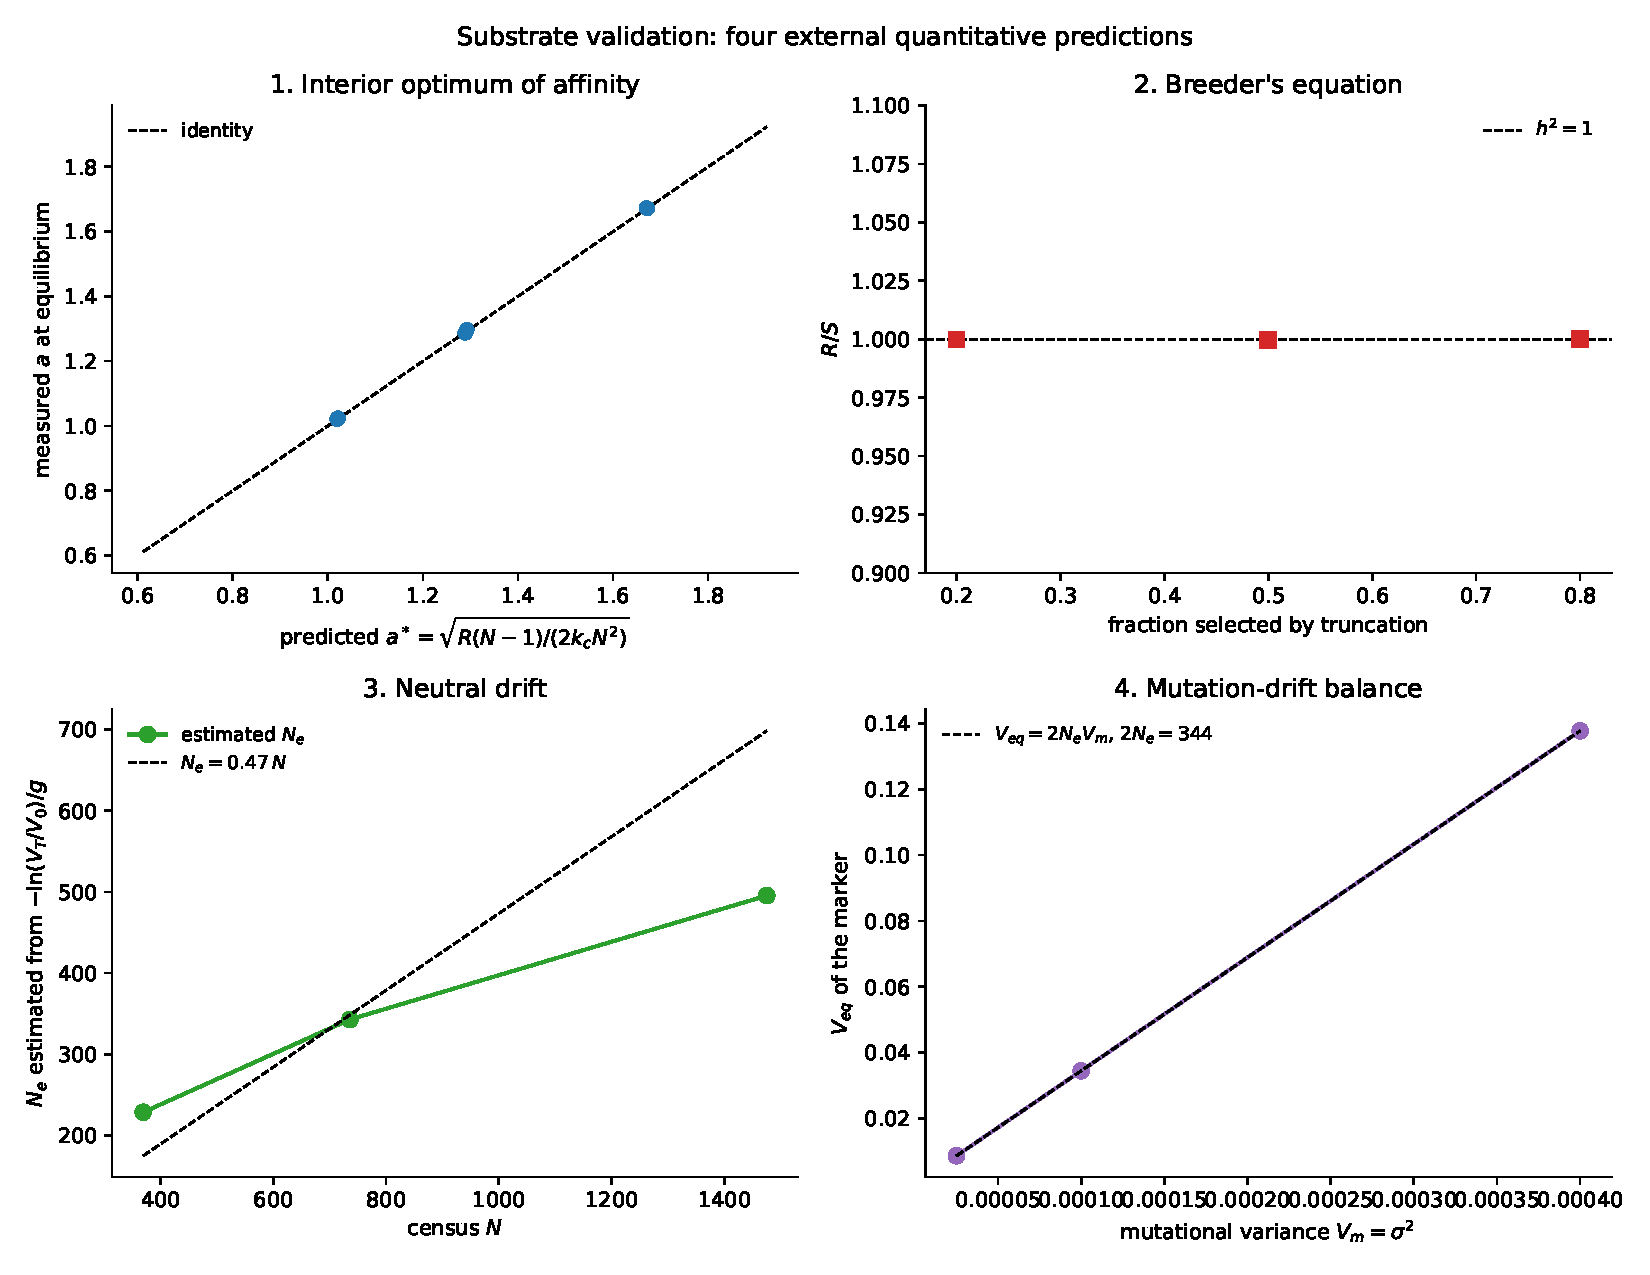
\includegraphics[width=0.94\linewidth]{fig_validacion}
\caption{Substrate validation against four external quantitative predictions: the analytic evolutionarily stable affinity, the breeder's equation, the relationship between effective and census population size, and the scaling of equilibrium marker variance with mutational variance.}
\label{fig:valid}
\end{figure}

\subsection{Neither coordinate has a dynamical signature at baseline}

In monoculture the four conditions are \textbf{bit-for-bit identical}:
same births, same deaths, same final population, same mean genome, in
100 of 100 seeds. This is a
determinism check rather than a statistical one---a seed either yields
four identical trajectories or it does not, and a single discrepancy
would falsify the claim---so it needs no interval and admits no
dispersion.

The reason is the one \eqref{eq:neq} exists to name. A rule conditioned on
the label has nobody to disfavour when everyone carries the same label, so
it reduces to its unconditioned form. And an extrinsic rule applying the
same criterion at the same moment as its intrinsic counterpart produces
the same allocations. \emph{The coordinates are properties of rules, not
of trajectories.} They are invisible until the intervention that
interrogates them is run---which is the substantive reason an audit
(\S4) cannot be replaced by watching a system behave.

\subsection{Each intervention responds to exactly one coordinate}

\begin{table}[ht]
\centering\small
\caption{The two interventions are orthogonal to each other. Withdrawing
the external operator moves only the control coordinate; relabelling the
recipient moves only the exchangeability coordinate. Point estimates with
95\% bootstrap intervals.}
\label{tab:orto}
\begin{tabular}{lccrr}
\toprule
\textbf{Condition} & $C$ & $A$ & \textbf{Operator removal} $\Phi_R/\Phi_B$ & \textbf{Relabelling} $L_1/L_0$\\
\midrule
$\mathrm{I/x}$ & I & 0 & 1.000~[0.993,\,1.007] & 0.989~[0.974,\,1.004]\\
$\mathrm{I/p}$ & I & 1 & 1.000~[0.993,\,1.007] & 0.000~[0.000,\,0.000]\\
$\mathrm{E/x}$ & E & 0 & 1.143~[1.134,\,1.152] & 0.989~[0.974,\,1.004]\\
$\mathrm{E/p}$ & E & 1 & 1.143~[1.134,\,1.152] & 0.000~[0.000,\,0.000]\\
\bottomrule
\end{tabular}
\end{table}

\begin{figure}[ht]
\centering
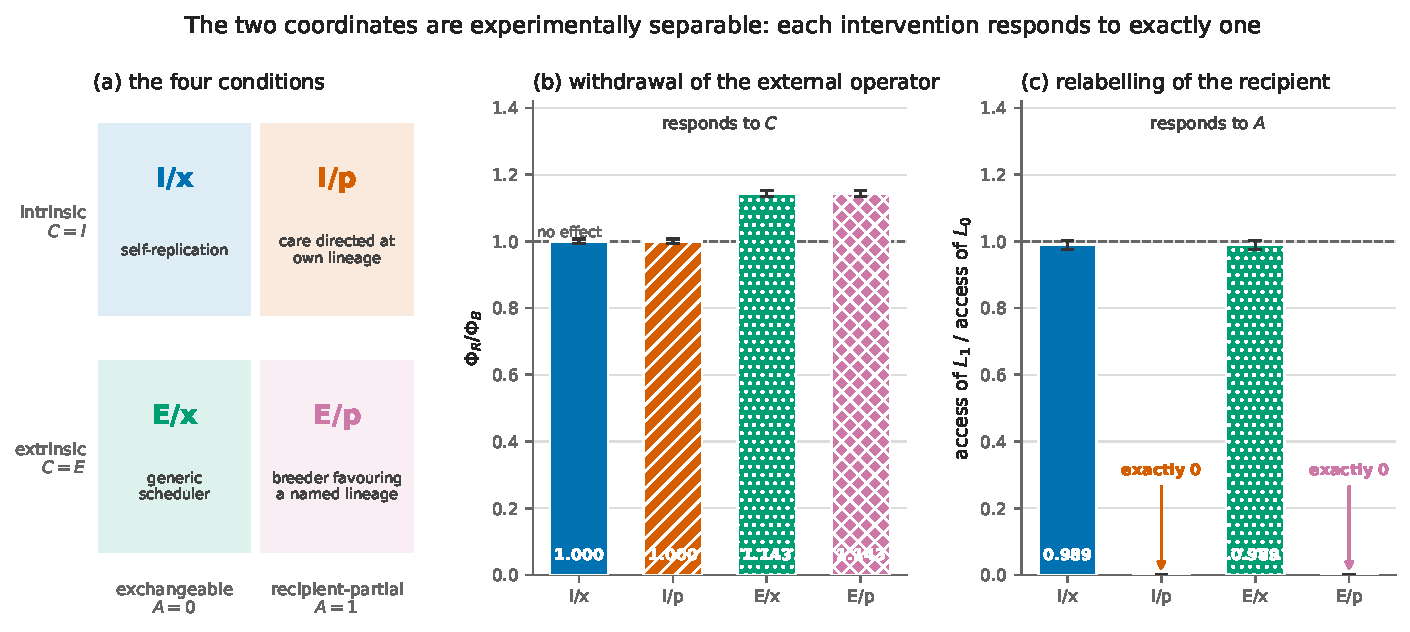
\includegraphics[width=1.0\linewidth]{fig1_ortogonalidad}
\caption{The two coordinates are experimentally separable. (a) The four conditions differ from their neighbours in exactly one thing. (b) Withdrawing the externally operated supply leaves the intrinsic conditions at exactly $1.000$ and moves both extrinsic ones. (c) Relabelling the recipient leaves the exchangeable conditions unchanged and drives allocation to the relabelled lineage to exactly zero in both partial ones. Bars carry 95\% bootstrap intervals; hatching encodes condition so identity never rests on colour alone.}
\label{fig:orto}
\end{figure}

Table~\ref{tab:orto} and Figure~\ref{fig:orto} are the experimental
content of \eqref{eq:twoaxes}. They are construct validation: the four
rules were built to differ in one thing each, so a clean separation is
partly a property of the design. What it establishes is that the
coordinates \emph{can} be manipulated independently, which was in doubt.
Withdrawing the externally operated supply leaves the two intrinsic
conditions at a ratio of exactly $1.000$ with zero dispersion across
seeds---there is no external machinery to withdraw---while both extrinsic
conditions move. Relabelling leaves the two exchangeable conditions
unchanged and drives allocation to the relabelled lineage to exactly zero
in both partial ones.

The zeros are worth dwelling on. They are not small numbers with
intervals that happen to include zero; they are exact, because the rule's
domain excludes the label and no sampling variation can put it back. A
binary $A$ is the honest report of a binary fact.

\subsection{Two things the framework got wrong}

Running the framework rather than only arguing it turned up two defects
in it. Both are reported here, in one place, because they are findings
of the experiment rather than caveats on it: the first concerns what the
exchangeability coordinate fails to distinguish, and the second, in
\S6.5, concerns the range of the normalized substitution contrast.
Neither is patched.

\paragraph{Exclusion and partition share a coordinate and have opposite
outcomes}
The two partial cells share a coordinate and behave in opposite ways, and
the framework as stated does not distinguish them.
Figure~\ref{fig:relabel} shows both panels of it.
Under $\mathrm{E/p}$ a single allocator conditioned on identity excludes:
the relabelled lineage receives nothing from anyone. Under
$\mathrm{I/p}$ each donor serves its own label, so the relabelled lineage
receives---but only from itself. Allocation across the label boundary is
exactly zero in both; aggregate supply to the relabelled lineage is zero
in one and positive in the other.

This is a genuine gap in the account of \S2, found by running it. The
coordinate $A$ answers whether a rule's allocation depends on recipient
identity. It does not answer whether the resulting partition leaves the
disfavoured lineage with a viable supply of its own, and those come apart
in the most ordinary case in biology: identity-keyed care partitions a
population without starving anybody's offspring but their own kin's
competitors. A graded $A$ may capture part of this distinction but is
not guaranteed to resolve it: the difference may be one of the topology
of the allocation rather than of the intensity of partiality.

\begin{figure}[ht]
\centering
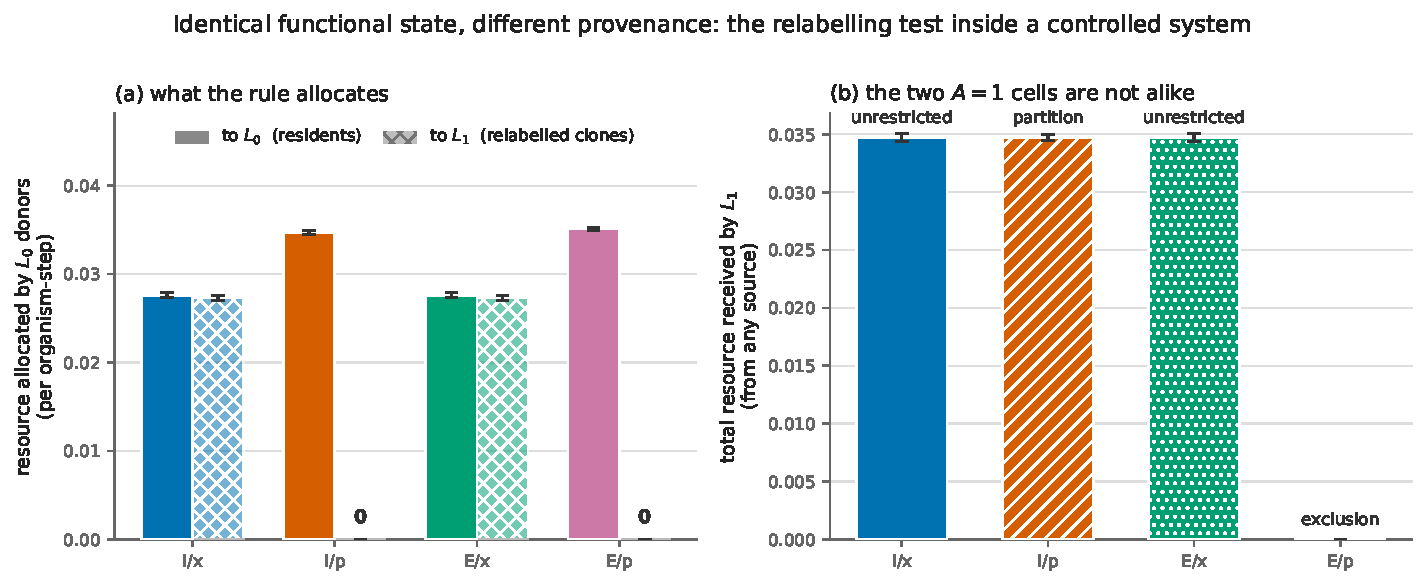
\includegraphics[width=0.92\linewidth]{fig2_reetiquetado}
\caption{Identical functional state, different provenance. (a) What the rule allocates to residents and to relabelled clones, per organism-step, in a short window after injection. (b) Total supply reaching the relabelled lineage from any source: the two $A=1$ cells share a coordinate and differ completely, one excluding and the other partitioning.}
\label{fig:relabel}
\end{figure}

\subsection{The range of \texorpdfstring{$\rho$}{rho}, what the data do not separate, and a principled \texttt{NA}}

\begin{table}[ht]
\centering\small
\caption{The three arms, at the largest competing-lineage size tested ($n_{L_1}=200$ of 400). $\Phi$ is autonomous reproductive cycles completed by the focal
lineage, with 95\% bootstrap intervals. Arm S is matched to arm B on
emitted volume for the resource manipulation; for the suppression
manipulation no defensible match exists and the entry is the range of
$\rho$ over the substitute's whole intensity range, for the reasons
given under matching. The acquisition cost paid in arm S is reported
separately and never absorbed into $\Phi$.}
\label{tab:brazos}
\begin{tabular}{lrrrcc}
\toprule
\textbf{Manipulation} & $\Phi_B$ & $\Phi_R$ & $\Phi_S$ & $\delta$ & $\rho$\\
\midrule
Partial transfer (negative control) & 149\,192 & 77\,389 & 78\,848 & +0.48 & 0.98~[0.82,\,1.19]\\
Reproductive resource & 168\,214 & 78\,848 & 80\,979 & +0.53 & 0.98~[0.86,\,1.11]\\
Competitor suppression & 151\,506 & 78\,848 & 85\,309 & +0.48 & 0.91--1.10\\
\bottomrule
\end{tabular}
\end{table}

Throughout this section $\rho$ is the normalized substitution contrast
of \eqref{eq:rho}, not a fraction: zero and one are reference points
and values above one are meaningful.

Table~\ref{tab:brazos} reports the three manipulations at the largest
competing-lineage size and Figure~\ref{fig:brazos} the raw continuity
values behind them; the dose-response below gives the rest. One
bookkeeping point, so that nothing is counted twice: the baseline and
removal arms of the first manipulation at $n_{L_1}=0$ are the same
measurement as the $\mathrm{E}$ rows of Table~\ref{tab:orto}, not an
independent replication of it.

\paragraph{The negative control, and a pre-registered prediction that
failed} We pre-registered that the partial transfer rule would return
$\rho=\texttt{NA}$ throughout, because the audit calls it
recipient-partial while baseline dependence on it is not positive. It
does so at $n_{L_1}\in\{0, 40\}$: at
$n_{L_1}=0$ the supply is a \emph{constraint} rather than a support
($\delta=-0.125$, withdrawing it raises
the autonomous cycle count---a property of the transfer being
externally operated rather than of its partiality, as \S6.6 sets out),
so there is no demonstrated dependence to
apportion and the honest output is not a number. That is \eqref{eq:neq}
measured rather than argued: $A=1$ with $\rho=\texttt{NA}$ is a real
state of affairs, and a method reporting $\rho=0$ there would turn the
absence of demonstrated dependence into a spurious estimate of
complete restoration.

At $n_{L_1}\in\{100, 200\}$ the
prediction fails, and the reason is worth more than the prediction
was. A partial allocation rule in a mixed population is not only a
support that might turn out to be unnecessary; it is also a
\emph{competitor-suppression mechanism}, because the non-focal
lineage contributes to the pool and is not served. Once the
competitor is large enough, withdrawing the rule releases it and
harms the focal lineage, so baseline dependence becomes positive.
The negative control and the suppression manipulation converge at
high dose---which is a finding about what partial allocation
\emph{is}, not a defect of either.

\paragraph{\texorpdfstring{$\rho$}{rho} above one: the second defect}
At $n_{L_1}=100$ the negative control returns
$\rho=1.66~[1.07,\,3.04]$, whose interval excludes one from
below---which the normalized substitution contrast permits, since
it is not a fraction and has no upper bound. $\rho>1$ means
$\Phi_S<\Phi_R$: de-personalising the rule costs the focal lineage more
than withdrawing it altogether, because the open substitute does not
merely stop favouring the focal lineage---it supplies the rivals the
partial rule was excluding. \S3.5 now states the unbounded range and
what values above one mean.

\paragraph{The range of \texorpdfstring{$\rho$}{rho}, and what the data do not separate}
The range is established within the resource manipulation, along the
dose, not by contrasting manipulations. At $n_{L_1}=0$
$\rho=-0.02~[-0.10,\,0.05]$ and at $n_{L_1}=200$
$\rho=0.98~[0.86,\,1.11]$; the two intervals are disjoint.
So the contrast moves from about its zero reference point to about its
one, driven by a quantity we control.

What the data do \emph{not} support is a separation between the
manipulations at the largest dose. There all three intervals cover one and every pair overlaps, so at
$n_{L_1}=200$ we cannot distinguish a rule whose benefit
was the resource from one whose benefit was the exemption. An
earlier run at thirty seeds appeared to separate them; it did not
survive the increase to 100. We report the
convergence rather than the appearance.

The convergence has a mechanism rather than being an artefact of the
estimator: as the competing lineage grows, what the partial provider
withholds from it becomes a larger part of what the focal lineage
enjoys, so supplying a resource and suppressing a competitor converge
on being the same intervention.

\paragraph{The dose-response, and where \texorpdfstring{\texttt{NA}}{NA} comes back}
Varying the size of the competing lineage moves $\rho$ systematically:
\begin{center}\small
\begin{tabular}{rccc}
\toprule
$n_{L_1}$ & Partial transfer & Reproductive resource & Competitor suppression\\
\midrule
0 & \texttt{NA} & -0.02 & \texttt{NA}\\
40 & \texttt{NA} & 0.50 & 0.92--1.73\\
100 & 1.66 & 0.85 & 0.91--1.27\\
200 & 0.98 & 0.98 & 0.91--1.10\\
\bottomrule
\end{tabular}
\end{center}

At $n_{L_1}=0$ the partial rule has nobody to disfavour and $\rho$ is
undefined in the two manipulations whose baseline dependence vanishes
there. That is the limiting case of the monoculture identity of \S6.2,
and it is the clearest statement the experiment produces:
\emph{partiality needs someone to disfavour before it can matter to
anything}.

The resource curve rises monotonically and approaches one from below rather than
plateauing short of it; an apparent plateau at thirty seeds did not
survive. The approach to one is expected here, since $\rho=1$ is the
point at which none of this manipulation's dependence survives
de-personalising the rule.

\paragraph{A support that was a constraint}
\S3.5 predicts that $\delta$ can be negative, and it is: at
$n_{L_1}=0$ the externally operated transfer
gives $\delta=-0.125~[-0.132,\,-0.118]$, strictly below zero,
and withdrawing it leaves the lineage completing about 14\% \emph{more} reproductive cycles. Table~\ref{tab:orto} gives the
identical ratio for $\mathrm{E/x}$ and $\mathrm{E/p}$, so the
constraint belongs to the transfer being \emph{operated from
outside} rather than to its partiality, and applies to both
extrinsic cells. The mechanism agrees: levelling reserves costs the
individuals closest to reproducing more than it gains those
furthest from it, which is about the allocation, not the label. A
framework reading every external supply as support would have
scored this one backwards; the sign of $\delta$ is what stops it.

\begin{figure}[ht]
\centering
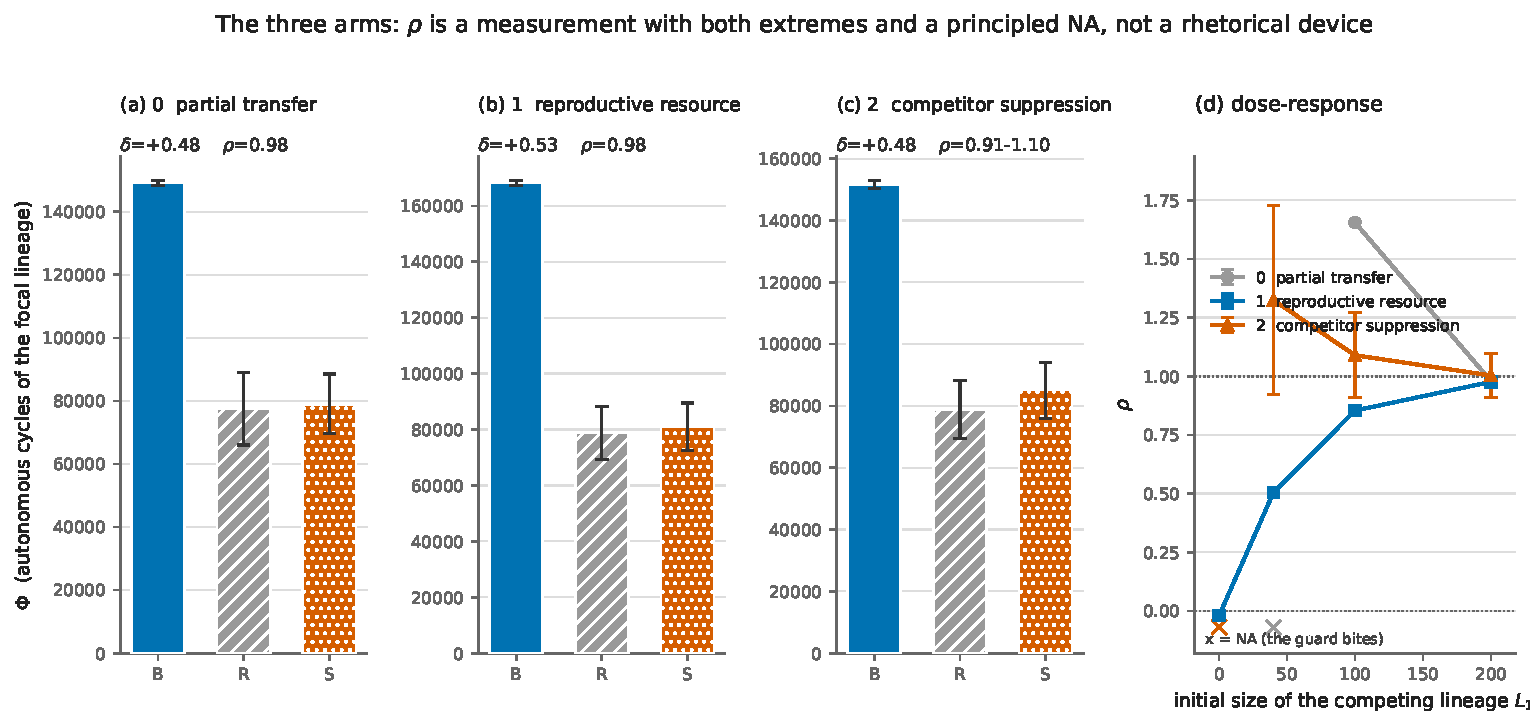
\includegraphics[width=1.0\linewidth]{fig3_brazos}
\caption{The three arms. (a)--(c) Raw continuity in each arm, which is the primary result; $\delta$ and $\rho$ are derived from it. (d) $\rho$ against the size of the competing lineage, with crosses marking the doses at which the guard bites and the honest output is \texttt{NA} rather than zero.}
\label{fig:brazos}
\end{figure}

\paragraph{Matching, and where we could not achieve it}
Calibration used pilot seeds disjoint from the confirmatory ones and was
discarded. For the provider the matched quantity is directly
controllable: at $n_{L_1}=200$ the substitute emitted 680\,083 units against a target of 680\,083 (0.0\% error). The acquisition cost recipients paid to qualify was 0.12 times the volume received; that is the price of an open rule and it
belongs in the report, not in $\Phi$.

For the suppression manipulation we could not construct a defensible
match, and say so rather than presenting one. The obvious target---the
fraction of reproduction the rule prevents---turned out to be unusable
twice over. A counter of blocked events counts organism-steps rather
than prevented events, and the partial rule sterilises a sublineage
permanently, so its blocked individuals accumulate in a way the open
rule's do not; the two arms inflate by different factors. Retargeting to
realised reproduction, which counts events once, the calibration
converges to within $0.2\%$---but onto a quantity that is nearly
\emph{insensitive} to the manipulation, because the world compensates:
total births move by under $3\%$ while the substitute's intensity
ranges over two orders of magnitude. Fractions that differ by $100\times$
match equally well, and choosing between them would be arbitrary.

Matching on an insensitive quantity is not matching. We therefore report
$\rho$ across the substitute's whole range instead of at one calibrated
point. It stays near one throughout, so the conclusion is robust to a
matching choice we do not know how to make uniquely. That is a weaker
claim than the pre-registered one and a more defensible one, and it is
recorded as a deviation in the pre-registration.

\subsection{Does the open rule play favourites in effect?}

An exchangeable rule can still serve a systematically
better-endowed subset. Under \eqref{eq:exch} that is not
partiality---the rule is symmetric under relabelling and its
behaviour tracks state---but it is the exact edge of the
criterion, so we measured it. Observing who is served at each
moment, the open rule's recipients hold 47\% more reserve than the unserved, show no detectable difference in
affinity (0.1\% less), and sit at the 0.50 energy percentile---the median, not
the top. The excluded are the 1.3\% below the qualifying threshold, overwhelmingly newborns, and
the exclusion is transient.
Under the partial rule the recipients instead hold 6.8\% less reserve than the unserved, selected on
a label no amount of reserve can change.
So the answer is no: the open rule gates on a state anyone
reaches rather than concentrating on the fittest, and the
distinction \S2.2 draws between state-dependence and
identity-dependence survives contact with the data.

\subsection{The audited systems as profiles}

Figure~\ref{fig:perfil} shows the audit of \S4 as one coordinate per
function per system, with no aggregation. Two things are legible in it
that a summary index would hide. The canonical genetic algorithm and
the population-evolved language models are identical cell by cell,
three decades apart: the coincidence is seen rather than asserted. And
incomparability is read by comparing rows---among the rows audited
here, no artificial one
dominates the replicator's and the sovereign agents' both, whichever
value the indeterminate entry takes, while the free-living population
dominates each of them, which is the comparison the biological rows are
there to provide. These eight systems are spread across the space of
profiles rather than ordered along one; whether evolutionary systems at
large are so spread is not something eight cases can settle.

\begin{figure}[ht]
\centering
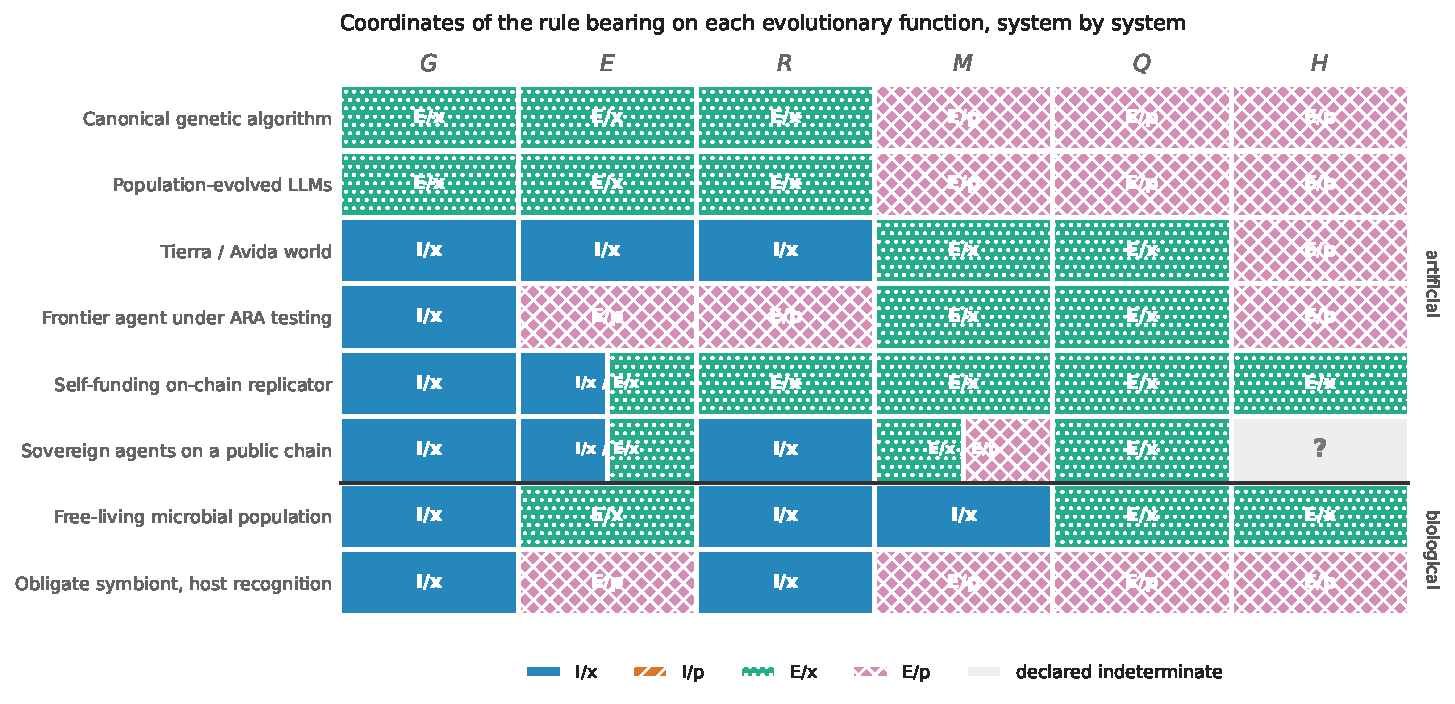
\includegraphics[width=1.0\linewidth]{fig4_perfil}
\caption{Each cell is the coordinate pair of the rule bearing on that function, transcribed from Table~\ref{tab:audit} and from nothing else. Split cells are functions served by two rules with different coordinates; the grey cell is the habitat entry declared indeterminate there. There are no numeric axes and no aggregation: \S2.5 gives no principled weights, so none are used.}
\label{fig:perfil}
\end{figure}

% ============================================================
\section{Scope}
% ============================================================

\paragraph{Open-endedness} A lineage can be exchangeably supplied and
generate almost no novelty, and a richly generative experiment can be
wholly partial \citep{taylor2016,banzhaf2016,packard2019}. The two may
interact---imposed evaluation constrains the reachable space, exchangeable
interaction can create new selective opportunity---but the relation is
empirical. Human culture is the instructive case: substantial dynamical
independence from genetic evolution \citep{borg2024} while every one of its
rules runs on biological minds.

\paragraph{Individuality} Whether humans and AI are becoming a
higher-level evolutionary individual \citep{rainey2023,raineyhochberg2025}
is a question about the boundary of $D$, not about either coordinate.

\paragraph{Life} We make no claim about it. No definition reliably
captures known life while admitting plausible novel forms
\citep{abbott2026,stepney2025}, and making the empirical question wait on
the ontological one is what has kept it unasked.

% ============================================================
\section{Limitations}
% ============================================================

\paragraph{Exchangeability is one dimension, and the state/label split
requires judgement} The central limitation is structural rather than a
caveat: a system may be exchangeably supplied throughout and wholly operated
from outside, so claims about evolutionary autonomy require both coordinates.
And the attainability criterion of \S2.2 removes much of the arbitrariness in
the split but not all of it, since what counts as available to a candidate is
a modelling choice and a substrate can be open in principle and closed in
practice. The split must be declared before analysis.

\paragraph{\texorpdfstring{$A$}{A} is binary, and does not distinguish exclusion from partition}
A graded version needs a distribution over configurations, one over
permutations and a metric on allocations, so we report a binary property
rather than a number we cannot defend. The coordinate also answers whether
allocation depends on recipient identity, not whether the resulting partition
leaves the disfavoured lineage a supply of its own; \S6.4 measures both, and a
graded $A$ might capture part of that distinction without resolving it, since
the difference may be one of allocation topology rather than intensity.

\paragraph{The orthogonality result is construct validation}
The four rules were written to differ in one thing each, so a clean separation
is partly a property of the design. It establishes that the framework can be
implemented causally, which was in doubt; it is not evidence about how the
coordinates separate in systems nobody built for the purpose. The
findings that do not come from our design are $\rho>1$, the convergence of the
two manipulations under competition, and exclusion versus partition.

\paragraph{\texorpdfstring{$\rho$}{rho} is relative to a declared matching, and is a ratio estimator}
Matching arm~S on emitted volume and on per-recipient rate are both defensible
and give different numbers, and for one manipulation no defensible match
exists (\S6.5), so $\rho$ is relative to a stated convention rather than a
property of the system. It is also unstable near its denominator's zero, which
is why \eqref{eq:rho} returns \texttt{NA} there, and arm~S is not always
constructible: for frontier agents a condition in which no trial is initiated
may be unsafe or unaffordable. The choice of interval estimator was examined
rather than assumed: an unpaired bootstrap, which ignores the correlation the
shared seeds induce, gives intervals up to fifteen per cent wider and changes
no conclusion reported here. At two dose points pairing widens the interval
instead, because the arms are negatively correlated there rather than
positively---a seed favourable to the baseline arm can be unfavourable to the
substitute---which is a property of those points and not an artefact of the
estimator. Both bootstraps are in the repository.

\paragraph{The audit rests on judgement, and never establishes importance}
Nothing guarantees that a system's mechanisms decompose cleanly into Taylor's
functions, and the shared-substrate criterion is a stipulation that must be
applied uniformly---a reader drawing the boundary elsewhere gets different
coordinates for the same system. Table~\ref{tab:audit} is not an autonomy
claim either. \S4.6 reads a running population off a published case study;
the relabelling test of \S3.2 would settle several entries, including the
indeterminate one.

\paragraph{The order is partial, and carries no normative verdict}
A reader wanting to know which of two systems is ``closer to autonomy'' will
not get an answer, which we take to be correct, not evasive: producing
one would require weights nothing in the framework supplies. Nor does anything
here imply that reduced partiality or increased intrinsic operation is
desirable. Commercial incentives push one way on the control axis while
pushing systems toward exchangeable supply on ours, which is itself a reason
to measure them separately.

% ============================================================
\section{Conclusion}
% ============================================================

Whether the supply a lineage receives depends on who that lineage is, rather
than on what state it is in, is a property of the organization of that supply,
and it is not the same question as who operates the rule. Biology settles the
two independently: a nutrient patch is external and anonymous, a host that
recognises particular symbionts is external and not. The second question --- who
sets the criteria and executes the loop --- is the one the field already has a
theory for. It is what ``domesticated,'' ``breeder regime'' and ``not yet
feral'' all point at, and \citet{taylor2019} formalised it as extrinsic
implementation. Artificial systems are where the first question has recently
begun to move, and where both become measurable.

What we claim is that a rule bearing on an evolutionary function has two
independent properties, that the field has a name and a theory for one of them,
and that the other characterises an under-examined change in increasingly
agentic systems. An agent renting compute from a market that does not know who
it is has moved on the second axis and not at all on the first. Reading that as
progress toward autonomy is a mistake; so is failing to notice it.

The audit returns a result we would put weight on. The partiality that
informal discussion attributes to imposed fitness functions is mostly not
there; what is there, in the genetic algorithm of the 1990s and the language-model
population of today alike, is extrinsic operation of evaluation and
reproduction.

The worked cases are sharper still. Among the systems audited here, three
artificial ones three decades apart go unranked by the two coordinates: a
digital organism
deeply intrinsic and inhabiting a world maintained for it; a smart contract
subject to no partial rule anywhere, which buys that with a replication
routine it neither owns nor can evolve; and a population of blockchain agents
that beats the contract on the core functions and would have dominated it on
every function the evidence settles, had its maintainers not stepped in to
defend their own offspring. That last
intervention is the paper in miniature: not a loss of intrinsic control, not
mere dependence, but the one thing in the loop that would not have been
available to a lineage that was not theirs---and the system's own authors
flagged it as a problem without a name for what kind of problem it was. A
framework tracking control alone puts these three in a line, and every
available ranking suppresses something true.

Running the framework produced one result we did not expect, and it is
negative: at baseline neither coordinate has any dynamical signature at all.
Four conditions differing in who operates a rule and in whether its domain
includes the recipient's label produce bit-for-bit identical trajectories, and
each becomes visible only under the intervention that interrogates it. That
settles what an audit is for. If the coordinates were readable off behaviour,
reading published specifications would be a poor substitute for watching
systems run. They are not, so it is not. It also produced two defects in our
own account, set out in \S6.4 and \S6.5 and left open rather than repaired.

If the interesting question is where a system's rules sit on two
coordinates rather than what the system can do, then external influence has
been tracked along only one of at least two dimensions on which it varies.

% ============================================================
\section*{Data and code availability}
% ============================================================

The simulation, the analysis pipeline, the pre-registration, every
% CONFIRMAR: hace falta una via de acceso PARA REVISION que no obligue al
% revisor a identificarse.  BioSystems usa revision simple ciego: no hay
% identidad de autor que proteger, pero si la del revisor, y un repositorio
% privado de GitHub solo admite colaboradores nombrados, de modo que pedir
% acceso por correo revela quien lo pide.  Ver envio/NOTAS_ENVIO.md.
configuration and every seed are available at \repourl. The repository is
administered by Ra\'ul-Antonio Ja\'en-Garc\'ia and is private until
publication; access is granted on request to editors and reviewers, at
\texttt{raul.jaen@edu.upct.es}. Each
result file is stored with a manifest recording the complete run
specifications, a hash of the source that produced it and the environment
versions, so no result is separable from the conditions that generated it.
Three properties are asserted in the repository's test suite rather than in its
prose: a run specification determines its output bit for bit; the output does
not depend on the number of parallel workers or on execution order; and the
bootstrap is seeded. The suite also parses Table~\ref{tab:audit} and re-derives
every dominance claim this paper makes about it. Pilot runs used for
calibration carry seeds disjoint from the confirmatory ones and are discarded.
Cohort and generation-interval measurements are reported in the supplementary
material, generated from the same result files as the main text.

% ============================================================
\section*{CRediT authorship contribution statement}
% ============================================================

\textbf{Ra\'ul-Antonio Ja\'en-Garc\'ia:} Conceptualization, Methodology,
Software, Formal analysis, Investigation, Data curation, Writing --- original
draft, Writing --- review \& editing, Visualization.
\textbf{Jorge Larrey-Ruiz:} Supervision.

% ============================================================
\section*{Funding}
% ============================================================

% CONFIRMAR: los autores confirman que no hubo financiacion especifica.
% Si la hubo, sustituir por la mencion exacta que exija el financiador.
This research did not receive any specific grant from funding agencies in the
public, commercial, or not-for-profit sectors.

% ============================================================
\section*{Declaration of generative AI and AI-assisted technologies in the
manuscript preparation process}
% ============================================================

% CONFIRMAR: los dos autores validan el alcance y firman la responsabilidad.
% Texto modelo de Elsevier, rellenado con las herramientas realmente usadas.
%
% PREGUNTA ABIERTA, a responder antes de enviar: aqui solo consta Anthropic
% Claude.  Si alguna OTRA herramienta generativa intervino en la preparacion
% del manuscrito --por ejemplo otros modelos de lenguaje usados para criticar
% borradores, si esas criticas se tradujeron en correcciones del texto--, debe
% figurar junto a Claude, nombrada y con para que se uso.  La declaracion no
% se aplica a correctores de gramatica y ortografia.  El texto de abajo se
% deja como esta hasta que los autores respondan.
During the preparation of this work the authors used Anthropic Claude in order
to draft and edit manuscript prose, to write and revise the simulation and
analysis code, and to generate the figures. After using this tool the authors
reviewed and edited the content as needed and take full responsibility for
the content of the published article.

\bibliographystyle{elsarticle-harv}
\bibliography{references}

\end{document}
